\documentclass[conference]{IEEEtran}
\IEEEoverridecommandlockouts

\usepackage[T1]{fontenc}
\usepackage{amsmath,amssymb}
\usepackage{xcolor}
\usepackage{tikz}
\usetikzlibrary{arrows.meta,positioning,fit,calc,backgrounds}

\begin{document}


\section{MileSE System Architecture}
\label{sec:architecture}
\subsection{Top-Level Overview}
MileSE is organized around a strict trust boundary. The untrusted advisory layer consists of the LLM planner and the milestone sequence it produces; these inputs may suggest promising intermediate states, but they are never allowed to decide feasibility. The trusted verification core starts with the SystemVerilog design and the target assertion, elaborates RTL with a PySlang frontend, extracts procedural control-flow graphs (CFGs), records combinational dependencies, and builds a per-instance symbolic execution context. When enabled, cone-of-influence (COI) pruning uses assertion expressions and milestone-related signals as seeds to remove logic that cannot affect the target property.

The central mechanism of MileSE is a solver-driven milestone scheduler. A milestone sequence, whether supplied as a JSON file or generated by an LLM planner, decomposes a deep target into intermediate RTL conditions such as reset release, FSM state transitions, handshake completion, or counter thresholds. MileSE does not treat these milestones as trusted constraints. Instead, each work item in the search queue carries its symbolic store, path condition, cycle index, and milestone progress. The priority function ranks work items by remaining milestones, elapsed cycles, and a lightweight data-flow distance to the next milestone, so states that make temporal progress are explored before legal but irrelevant continuations.

Formal checking remains separated from heuristic guidance. During execution, branch feasibility, milestone satisfiability, and assertion violation checks are all discharged by Z3 over the current symbolic path condition. Milestones are checked observationally using solver scopes, so an unsatisfiable or malformed milestone is discarded rather than injected into the path condition. To tolerate imperfect plans, MileSE combines compound-condition parsing, conservative sliding-window lookahead, expected-cycle local bounds, lazy forking of alternative CFG paths, and targeted recomputation of derived combinational signals. As a result, LLM-generated or manually written milestones guide the order of exploration, while the symbolic executor and SMT solver remain responsible for semantic validity and counterexample construction.

\begin{figure*}[t]
    \centering
    \resizebox{\textwidth}{!}{%
    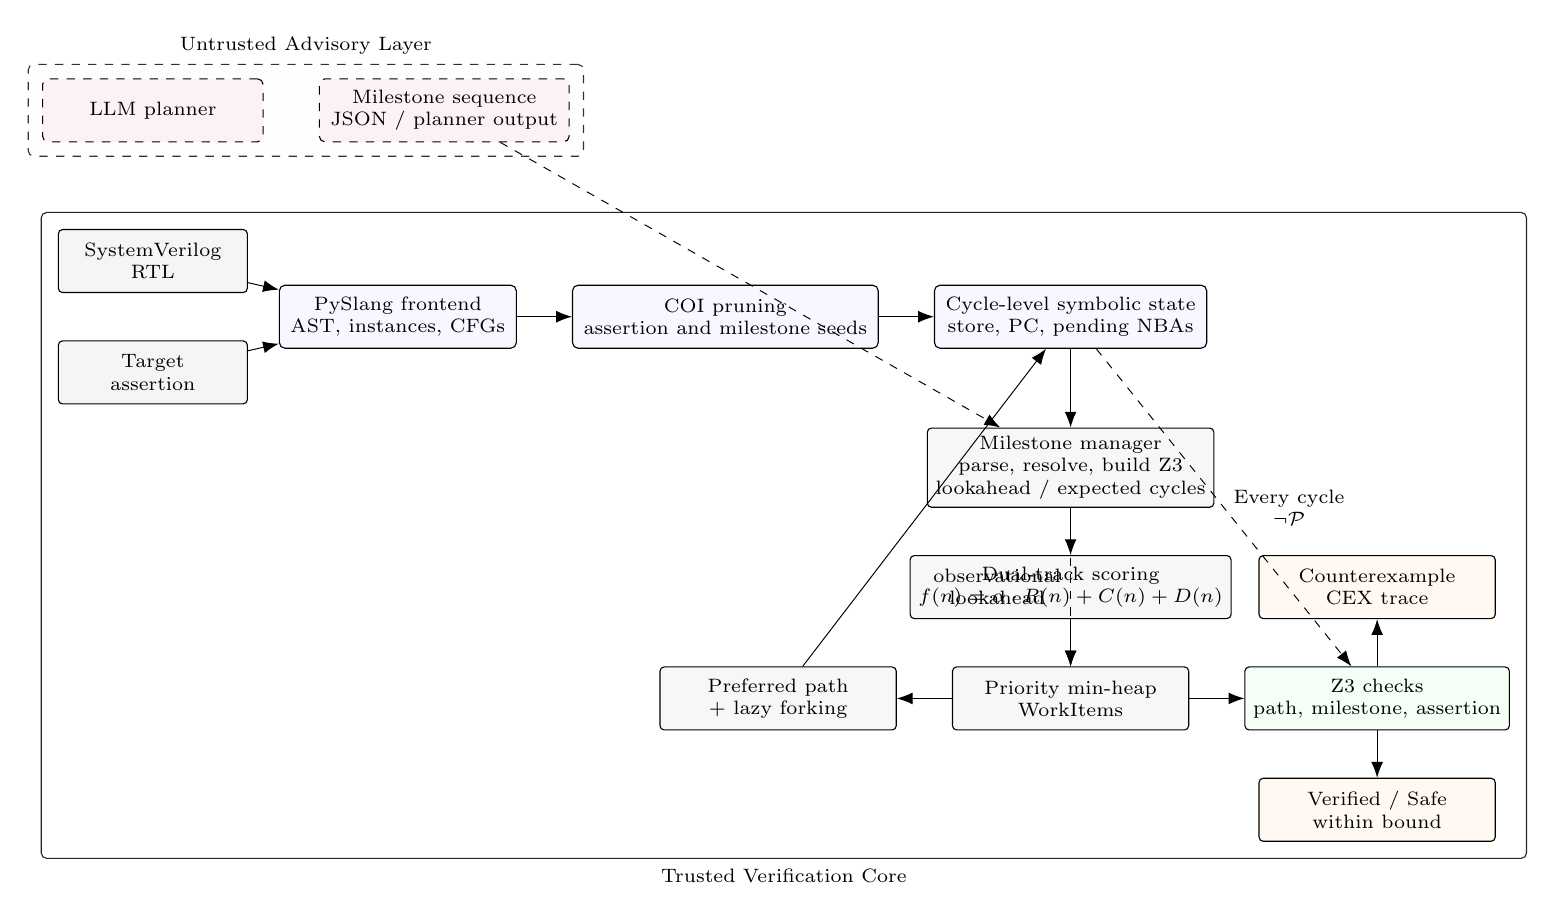
\begin{tikzpicture}[
        font=\scriptsize,
        node distance=6mm and 7mm,
        block/.style={
            draw,
            rounded corners=1.5pt,
            align=center,
            minimum height=8mm,
            minimum width=24mm,
            inner sep=3pt,
            fill=gray!8
        },
        advisory/.style={
            draw,
            dashed,
            rounded corners=2pt,
            align=center,
            minimum height=8mm,
            minimum width=28mm,
            inner sep=4pt,
            fill=purple!5
        },
        trusted/.style={
            draw,
            rounded corners=2pt,
            align=center,
            minimum height=8mm,
            minimum width=30mm,
            inner sep=4pt,
            fill=blue!3
        },
        guard/.style={
            draw,
            rounded corners=1.5pt,
            align=center,
            minimum height=8mm,
            minimum width=30mm,
            inner sep=3pt,
            fill=gray!6
        },
        solver/.style={
            draw,
            rounded corners=1.5pt,
            align=center,
            minimum height=8mm,
            minimum width=28mm,
            inner sep=3pt,
            fill=green!4
        },
        output/.style={
            draw,
            rounded corners=1.5pt,
            align=center,
            minimum height=8mm,
            minimum width=30mm,
            inner sep=3pt,
            fill=orange!5
        },
        flow/.style={-{Latex[length=2mm]}, line width=0.35pt},
        softflow/.style={-{Latex[length=2mm]}, line width=0.35pt, dashed}
    ]

    \node[advisory] (planner) {LLM planner};
    \node[advisory, right=of planner] (milestones) {Milestone sequence\\JSON / planner output};
    \begin{scope}[on background layer]
        \node[draw, dashed, rounded corners=2pt, fit=(planner)(milestones), inner sep=5pt,
              label={[font=\scriptsize]above:Untrusted Advisory Layer}, fill=purple!3, fill opacity=0.12, draw opacity=0.8] (advisorybox) {};
    \end{scope}

    \node[block, below=11mm of planner] (rtl) {SystemVerilog\\RTL};
    \node[block, below=of rtl] (assert) {Target\\assertion};
    \node[trusted, right=16mm of $(rtl)!0.5!(assert)$] (frontend) {PySlang frontend\\AST, instances, CFGs};
    \node[trusted, right=of frontend] (coi) {COI pruning\\assertion and milestone seeds};
    \node[trusted, right=of coi] (state) {Cycle-level symbolic state\\store, PC, pending NBAs};

    \node[guard, below=10mm of state] (manager) {Milestone manager\\parse, resolve, build Z3\\lookahead / expected cycles};
    \node[guard, below=of manager] (score) {Dual-track scoring\\$f(n)=\alpha \cdot R(n)+C(n)+D(n)$};
    \node[guard, below=of score] (queue) {Priority min-heap\\WorkItems};
    \node[guard, left=of queue] (fork) {Preferred path\\+ lazy forking};
    \node[solver, right=of queue] (z3) {Z3 checks\\path, milestone, assertion};
    \node[output, above=of z3] (cex) {Counterexample\\CEX trace};
    \node[output, below=of z3] (safe) {Verified / Safe\\within bound};

    \begin{scope}[on background layer]
        \node[draw, rounded corners=2pt, fit=(rtl)(assert)(frontend)(coi)(state)(manager)(score)(queue)(fork)(z3)(cex)(safe),
              inner sep=6pt, label={[font=\scriptsize]below:Trusted Verification Core}, fill=blue!2, fill opacity=0.08, draw opacity=0.85] (corebox) {};
    \end{scope}

    \draw[flow] (rtl) -- (frontend);
    \draw[flow] (assert) -- (frontend);
    \draw[flow] (frontend) -- (coi);
    \draw[flow] (coi) -- (state);
    \draw[softflow] (milestones) -- (manager);
    \draw[flow] (state) -- (manager);
    \draw[flow] (manager) -- (score);
    \draw[flow] (score) -- (queue);
    \draw[flow] (queue) -- (fork);
    \draw[flow] (fork) -- (state);
    \draw[flow] (queue) -- (z3);
    \draw[softflow] (state) -- node[midway,right,align=center]{Every cycle\\$\neg \mathcal{P}$} (z3);
    \draw[flow] (z3) -- (cex);
    \draw[flow] (z3) -- (safe);
    \draw[softflow] (manager) -- node[midway,left,align=center]{observational\\lookahead} (queue);

    \end{tikzpicture}%
    }
    \caption{Top-level MileSE workflow. The untrusted advisory layer proposes milestone sequences, while the trusted verification core elaborates RTL, prunes irrelevant logic, schedules work items, and discharges all feasibility and assertion checks through Z3.}
    \label{fig:milese_overview}
\end{figure*}
\end{document}
